% Options for packages loaded elsewhere
\PassOptionsToPackage{unicode}{hyperref}
\PassOptionsToPackage{hyphens}{url}
%
\documentclass[
  9pt,
  ignorenonframetext,
]{beamer}
\usepackage{pgfpages}
\setbeamertemplate{caption}[numbered]
\setbeamertemplate{caption label separator}{: }
\setbeamercolor{caption name}{fg=normal text.fg}
\beamertemplatenavigationsymbolsempty
% Prevent slide breaks in the middle of a paragraph
\widowpenalties 1 10000
\raggedbottom
\setbeamertemplate{part page}{
  \centering
  \begin{beamercolorbox}[sep=16pt,center]{part title}
    \usebeamerfont{part title}\insertpart\par
  \end{beamercolorbox}
}
\setbeamertemplate{section page}{
  \centering
  \begin{beamercolorbox}[sep=12pt,center]{part title}
    \usebeamerfont{section title}\insertsection\par
  \end{beamercolorbox}
}
\setbeamertemplate{subsection page}{
  \centering
  \begin{beamercolorbox}[sep=8pt,center]{part title}
    \usebeamerfont{subsection title}\insertsubsection\par
  \end{beamercolorbox}
}
\AtBeginPart{
  \frame{\partpage}
}
\AtBeginSection{
  \ifbibliography
  \else
    \frame{\sectionpage}
  \fi
}
\AtBeginSubsection{
  \frame{\subsectionpage}
}
\usepackage{lmodern}
\usepackage{amssymb,amsmath}
\usepackage{ifxetex,ifluatex}
\ifnum 0\ifxetex 1\fi\ifluatex 1\fi=0 % if pdftex
  \usepackage[T1]{fontenc}
  \usepackage[utf8]{inputenc}
  \usepackage{textcomp} % provide euro and other symbols
\else % if luatex or xetex
  \usepackage{unicode-math}
  \defaultfontfeatures{Scale=MatchLowercase}
  \defaultfontfeatures[\rmfamily]{Ligatures=TeX,Scale=1}
\fi
\usetheme[]{Berkeley}
\usecolortheme{dove}
\usefonttheme{structurebold}
% Use upquote if available, for straight quotes in verbatim environments
\IfFileExists{upquote.sty}{\usepackage{upquote}}{}
\IfFileExists{microtype.sty}{% use microtype if available
  \usepackage[]{microtype}
  \UseMicrotypeSet[protrusion]{basicmath} % disable protrusion for tt fonts
}{}
\makeatletter
\@ifundefined{KOMAClassName}{% if non-KOMA class
  \IfFileExists{parskip.sty}{%
    \usepackage{parskip}
  }{% else
    \setlength{\parindent}{0pt}
    \setlength{\parskip}{6pt plus 2pt minus 1pt}}
}{% if KOMA class
  \KOMAoptions{parskip=half}}
\makeatother
\usepackage{xcolor}
\IfFileExists{xurl.sty}{\usepackage{xurl}}{} % add URL line breaks if available
\IfFileExists{bookmark.sty}{\usepackage{bookmark}}{\usepackage{hyperref}}
\hypersetup{
  pdftitle={Pesquisa reproduzível},
  pdfauthor={Frederico Bertholini},
  hidelinks,
  pdfcreator={LaTeX via pandoc}}
\urlstyle{same} % disable monospaced font for URLs
\newif\ifbibliography
\usepackage{color}
\usepackage{fancyvrb}
\newcommand{\VerbBar}{|}
\newcommand{\VERB}{\Verb[commandchars=\\\{\}]}
\DefineVerbatimEnvironment{Highlighting}{Verbatim}{commandchars=\\\{\}}
% Add ',fontsize=\small' for more characters per line
\usepackage{framed}
\definecolor{shadecolor}{RGB}{248,248,248}
\newenvironment{Shaded}{\begin{snugshade}}{\end{snugshade}}
\newcommand{\AlertTok}[1]{\textcolor[rgb]{0.94,0.16,0.16}{#1}}
\newcommand{\AnnotationTok}[1]{\textcolor[rgb]{0.56,0.35,0.01}{\textbf{\textit{#1}}}}
\newcommand{\AttributeTok}[1]{\textcolor[rgb]{0.77,0.63,0.00}{#1}}
\newcommand{\BaseNTok}[1]{\textcolor[rgb]{0.00,0.00,0.81}{#1}}
\newcommand{\BuiltInTok}[1]{#1}
\newcommand{\CharTok}[1]{\textcolor[rgb]{0.31,0.60,0.02}{#1}}
\newcommand{\CommentTok}[1]{\textcolor[rgb]{0.56,0.35,0.01}{\textit{#1}}}
\newcommand{\CommentVarTok}[1]{\textcolor[rgb]{0.56,0.35,0.01}{\textbf{\textit{#1}}}}
\newcommand{\ConstantTok}[1]{\textcolor[rgb]{0.00,0.00,0.00}{#1}}
\newcommand{\ControlFlowTok}[1]{\textcolor[rgb]{0.13,0.29,0.53}{\textbf{#1}}}
\newcommand{\DataTypeTok}[1]{\textcolor[rgb]{0.13,0.29,0.53}{#1}}
\newcommand{\DecValTok}[1]{\textcolor[rgb]{0.00,0.00,0.81}{#1}}
\newcommand{\DocumentationTok}[1]{\textcolor[rgb]{0.56,0.35,0.01}{\textbf{\textit{#1}}}}
\newcommand{\ErrorTok}[1]{\textcolor[rgb]{0.64,0.00,0.00}{\textbf{#1}}}
\newcommand{\ExtensionTok}[1]{#1}
\newcommand{\FloatTok}[1]{\textcolor[rgb]{0.00,0.00,0.81}{#1}}
\newcommand{\FunctionTok}[1]{\textcolor[rgb]{0.00,0.00,0.00}{#1}}
\newcommand{\ImportTok}[1]{#1}
\newcommand{\InformationTok}[1]{\textcolor[rgb]{0.56,0.35,0.01}{\textbf{\textit{#1}}}}
\newcommand{\KeywordTok}[1]{\textcolor[rgb]{0.13,0.29,0.53}{\textbf{#1}}}
\newcommand{\NormalTok}[1]{#1}
\newcommand{\OperatorTok}[1]{\textcolor[rgb]{0.81,0.36,0.00}{\textbf{#1}}}
\newcommand{\OtherTok}[1]{\textcolor[rgb]{0.56,0.35,0.01}{#1}}
\newcommand{\PreprocessorTok}[1]{\textcolor[rgb]{0.56,0.35,0.01}{\textit{#1}}}
\newcommand{\RegionMarkerTok}[1]{#1}
\newcommand{\SpecialCharTok}[1]{\textcolor[rgb]{0.00,0.00,0.00}{#1}}
\newcommand{\SpecialStringTok}[1]{\textcolor[rgb]{0.31,0.60,0.02}{#1}}
\newcommand{\StringTok}[1]{\textcolor[rgb]{0.31,0.60,0.02}{#1}}
\newcommand{\VariableTok}[1]{\textcolor[rgb]{0.00,0.00,0.00}{#1}}
\newcommand{\VerbatimStringTok}[1]{\textcolor[rgb]{0.31,0.60,0.02}{#1}}
\newcommand{\WarningTok}[1]{\textcolor[rgb]{0.56,0.35,0.01}{\textbf{\textit{#1}}}}
\setlength{\emergencystretch}{3em} % prevent overfull lines
\providecommand{\tightlist}{%
  \setlength{\itemsep}{0pt}\setlength{\parskip}{0pt}}
\setcounter{secnumdepth}{5}

\title{Pesquisa reproduzível}
\subtitle{Métodos Quantitativos Aplicados à Ciência Política}
\author{Frederico Bertholini}
\date{05.out.2020}

\begin{document}
\frame{\titlepage}

\begin{frame}[allowframebreaks]
  \tableofcontents[hideallsubsections]
\end{frame}
\hypertarget{nunca-esqueuxe7a}{%
\section{Nunca esqueça}\label{nunca-esqueuxe7a}}

\begin{frame}[fragile]{Pacotes e diretório de trabalho}
\protect\hypertarget{pacotes-e-diretuxf3rio-de-trabalho}{}
\begin{Shaded}
\begin{Highlighting}[]
\CommentTok{\# rotina para carregar pacotes}
\NormalTok{lista.de.pacotes =}\StringTok{ }\KeywordTok{c}\NormalTok{(}\StringTok{"tidyverse"}\NormalTok{,}\StringTok{"haven"}\NormalTok{,}\StringTok{"lubridate"}\NormalTok{,}
                     \StringTok{"janitor"}\NormalTok{,}\StringTok{"readxl"}\NormalTok{,}
                     \StringTok{"stringr"}\NormalTok{, }\StringTok{"magrittr"}\NormalTok{,}
                     \StringTok{"survey"}\NormalTok{,}\StringTok{"srvyr"}\NormalTok{) }
                     

\NormalTok{novos.pacotes \textless{}{-}}\StringTok{ }
\StringTok{  }\NormalTok{lista.de.pacotes[}\OperatorTok{!}\NormalTok{(lista.de.pacotes }\OperatorTok{\%in\%}
\StringTok{                      }\KeywordTok{installed.packages}\NormalTok{()[,}\StringTok{"Package"}\NormalTok{])]}

\ControlFlowTok{if}\NormalTok{(}\KeywordTok{length}\NormalTok{(novos.pacotes) }\OperatorTok{\textgreater{}}\StringTok{ }\DecValTok{0}\NormalTok{) \{}\KeywordTok{install.packages}\NormalTok{(novos.pacotes)\}}

\KeywordTok{lapply}\NormalTok{(lista.de.pacotes, require, }\DataTypeTok{character.only=}\NormalTok{T)}

\KeywordTok{rm}\NormalTok{(}\DataTypeTok{list =} \KeywordTok{ls}\NormalTok{())}
\KeywordTok{gc}\NormalTok{()}


\CommentTok{\# Definindo o diretorio de trabalho como do arquivo local}
\KeywordTok{setwd}\NormalTok{(}\KeywordTok{dirname}\NormalTok{(rstudioapi}\OperatorTok{::}\KeywordTok{getActiveDocumentContext}\NormalTok{()}\OperatorTok{$}\NormalTok{path))}
\end{Highlighting}
\end{Shaded}
\end{frame}

\hypertarget{recapitulando-manipulauxe7uxe3o}{%
\section{Recapitulando
manipulação}\label{recapitulando-manipulauxe7uxe3o}}

\begin{frame}{Live coding de manipulação de dados}
\protect\hypertarget{live-coding-de-manipulauxe7uxe3o-de-dados}{}
Reproduzindo trabalho sobre COVID e estados
\end{frame}

\begin{frame}[fragile]{Exemplo de join}
\protect\hypertarget{exemplo-de-join}{}
\begin{Shaded}
\begin{Highlighting}[]
\KeywordTok{library}\NormalTok{(tidyverse)}

\NormalTok{A \textless{}{-}}\StringTok{ }\KeywordTok{tibble}\NormalTok{(}\DataTypeTok{Partido=}\KeywordTok{c}\NormalTok{(}\StringTok{"X"}\NormalTok{,}\StringTok{"Y"}\NormalTok{,}\StringTok{"Z"}\NormalTok{,}\StringTok{"Z"}\NormalTok{,}\StringTok{"W"}\NormalTok{),}
            \DataTypeTok{Estado=}\KeywordTok{c}\NormalTok{(}\StringTok{"Estado A"}\NormalTok{,}\StringTok{"Estado A"}\NormalTok{,}\StringTok{"Estado B"}\NormalTok{,}\StringTok{"Estado A"}\NormalTok{,}\StringTok{"Estado B"}\NormalTok{))}

\NormalTok{B \textless{}{-}}\StringTok{ }\KeywordTok{tibble}\NormalTok{(}\DataTypeTok{Estado=}\KeywordTok{c}\NormalTok{(}\StringTok{"Estado A"}\NormalTok{,}\StringTok{"Estado B"}\NormalTok{,}\StringTok{"Estado C"}\NormalTok{),}
            \DataTypeTok{Sigla =} \KeywordTok{c}\NormalTok{(}\StringTok{"A"}\NormalTok{,}\StringTok{"B"}\NormalTok{,}\StringTok{"C"}\NormalTok{))}

\NormalTok{C \textless{}{-}}\StringTok{ }\NormalTok{A }\OperatorTok{\%\textgreater{}\%}\StringTok{ }\KeywordTok{left\_join}\NormalTok{(B)}
\end{Highlighting}
\end{Shaded}

\begin{verbatim}
## Joining, by = "Estado"
\end{verbatim}

\begin{Shaded}
\begin{Highlighting}[]
\NormalTok{D \textless{}{-}}\StringTok{ }\NormalTok{A }\OperatorTok{\%\textgreater{}\%}\StringTok{ }\KeywordTok{full\_join}\NormalTok{(B)}
\end{Highlighting}
\end{Shaded}

\begin{verbatim}
## Joining, by = "Estado"
\end{verbatim}
\end{frame}

\begin{frame}[fragile]{\texttt{left\_join}}
\protect\hypertarget{left_join}{}
\begin{Shaded}
\begin{Highlighting}[]
\NormalTok{C}
\end{Highlighting}
\end{Shaded}

\begin{verbatim}
## # A tibble: 5 x 3
##   Partido Estado   Sigla
##   <chr>   <chr>    <chr>
## 1 X       Estado A A    
## 2 Y       Estado A A    
## 3 Z       Estado B B    
## 4 Z       Estado A A    
## 5 W       Estado B B
\end{verbatim}
\end{frame}

\begin{frame}[fragile]{\texttt{full\_join} (não fazer)}
\protect\hypertarget{full_join-nuxe3o-fazer}{}
\begin{Shaded}
\begin{Highlighting}[]
\NormalTok{D}
\end{Highlighting}
\end{Shaded}

\begin{verbatim}
## # A tibble: 6 x 3
##   Partido Estado   Sigla
##   <chr>   <chr>    <chr>
## 1 X       Estado A A    
## 2 Y       Estado A A    
## 3 Z       Estado B B    
## 4 Z       Estado A A    
## 5 W       Estado B B    
## 6 <NA>    Estado C C
\end{verbatim}
\end{frame}

\hypertarget{pesquisa-reproduzuxedvel}{%
\section{Pesquisa reproduzível}\label{pesquisa-reproduzuxedvel}}

\begin{frame}{Por quê?}
\protect\hypertarget{por-quuxea}{}
\begin{itemize}
\item
  Pra ciência
\item
  Pra você
\end{itemize}
\end{frame}

\begin{frame}{Ferramentas}
\protect\hypertarget{ferramentas}{}
\begin{itemize}
\item
  R e RStudio (ok)
\item
  Github
\item
  knitr e rmarkdown
\item
  LaTeX
\end{itemize}
\end{frame}

\begin{frame}{Fluxo de trabalho}
\protect\hypertarget{fluxo-de-trabalho}{}
\begin{enumerate}
\item
  Coleta
\item
  Análise
\item
  Comunicação
\end{enumerate}
\end{frame}

\begin{frame}{}
\protect\hypertarget{section}{}
\begin{center}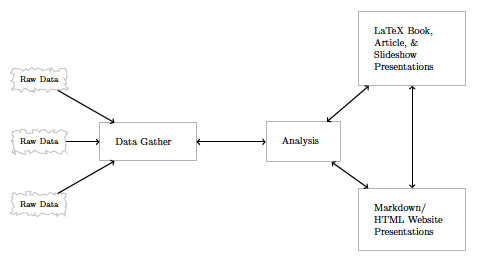
\includegraphics[width=1\linewidth]{imgs/fluxo_gandrud} \end{center}
\end{frame}

\begin{frame}{Dicas}
\protect\hypertarget{dicas}{}
\begin{enumerate}
\item
  Documente tudo!
\item
  Tudo é um arquivo (de texto).
\item
  Todos os arquivos devem ser legíveis (por humanos).
\item
  Relacione explicitamente seus arquivos.
\item
  Tenha um plano para organizar, armazenar e disponibilizar seus
  arquivos.
\end{enumerate}
\end{frame}

\begin{frame}{Trabalhando com projetos}
\protect\hypertarget{trabalhando-com-projetos}{}
Gerenciamento de arquivos: caminhos relativos e não absolutos

\begin{itemize}
\tightlist
\item
  Onde guardar seus projetos?
\end{itemize}
\end{frame}

\hypertarget{versionando-projetos}{%
\section{Versionando projetos}\label{versionando-projetos}}

\begin{frame}{}
\protect\hypertarget{section-1}{}
\begin{center}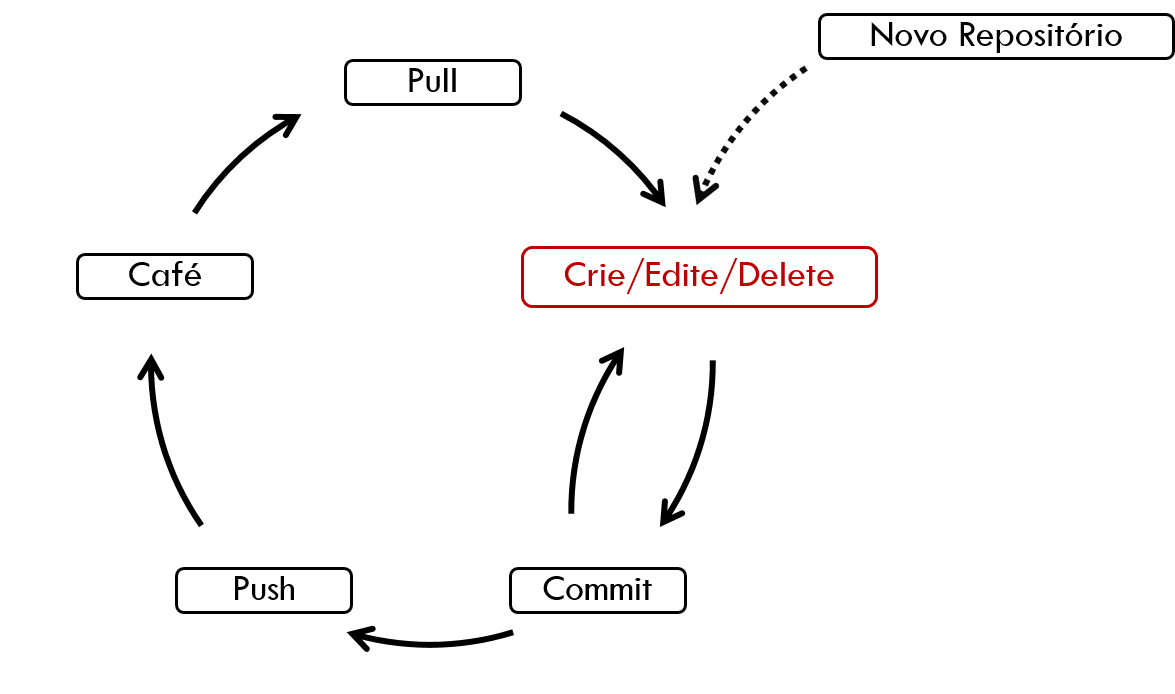
\includegraphics[width=0.8\linewidth]{imgs/fluxo_github_rstudio} \end{center}
\end{frame}

\begin{frame}{Passo-a-passo}
\protect\hypertarget{passo-a-passo}{}
\begin{enumerate}
\item
  Repositório: Criação de repositório do projeto no Github
\item
  .Rproj: Criação do Projeto no RStudio
\item
  Commit: Editando e ``Commitando'' as mudanças no código
\item
  Push: Subindo os commits para o Github
\item
  Pull: Baixando o estado atual do projeto
\end{enumerate}
\end{frame}

\begin{frame}{Caso tenha dificuldade}
\protect\hypertarget{caso-tenha-dificuldade}{}
\href{https://beatrizmilz.github.io/RLadies-Git-RStudio-2019/\#1}{Beatriz
Milz - RLadies}

\href{https://www.curso-r.com/blog/2017-07-17-rstudio-e-github/}{Curso
R}
\end{frame}

\end{document}
